\documentclass{article}
\usepackage[T1]{fontenc}
\usepackage{lmodern}
\usepackage{graphicx}
\usepackage{amsmath,amssymb}
\usepackage[a4paper,margin=2cm]{geometry}
\usepackage[absolute,overlay]{textpos}
\setlength{\TPHorizModule}{1mm}
\setlength{\TPVertModule}{1mm}
\usepackage[indonesian]{babel}
\usepackage{hyperref}
\setlength{\emergencystretch}{2em}
% unit: Halaman 24

\begin{document}

% === Halaman 24 (llm) ===

\begin{itemize}
  \item Luaran proses substitusi adalah blok $B$ yang panjangnya 32 bit.
  \item Blok $B$ menjadi masukan untuk proses permutasi.
  \item Tujuan permutasi adalah untuk mengacak hasil proses substitusi kotak-S.
  \item Permutasi dilakukan dengan menggunakan matriks permutasi $P$ (P-box) sbb:
\end{itemize}

\vspace{10mm}

\begin{center}
\begin{tabular}{|c|c|c|c|c|c|c|c|c|c|c|c|c|c|c|c|}
\hline
16 & 7 & 20 & 21 & 29 & 12 & 28 & 17 & 1 & 15 & 23 & 26 & 5 & 8 & 31 & 10 \\ \hline
2 & 8 & 24 & 14 & 32 & 27 & 3 & 9 & 19 & 13 & 30 & 6 & 22 & 11 & 4 & 25 \\ \hline
\end{tabular}
\end{center}

% deskripsi: Diagram alur proses kriptografi yang menunjukkan langkah-langkah dari input R_{i-1}, ekspansi menjadi 48 bit, fungsi E, operasi XOR dengan K_i menghasilkan A, substitusi melalui S-box menjadi blok B, dan terakhir proses permutasi P(B).
% bbox normalisasi: [0.6600, 0.6000, 0.9900, 0.8300]
\begin{textblock*}{69.30mm}(138.60mm,178.20mm)
\noindent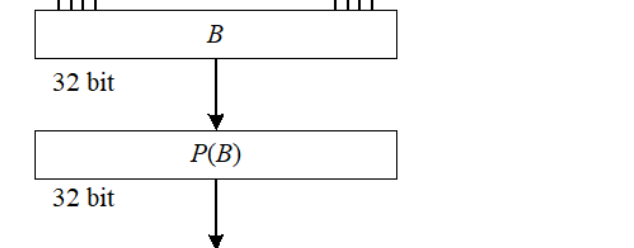
\includegraphics[width=69.30mm,height=68.31mm]{../../images/llm/page_024_img_01.png}%
\end{textblock*}

\end{document}
